\documentclass{../../test-template}

\begin{document}

\begin{center}
    \textbf{\Huge{Homework №3.} \\ \large Ентропія. ЛРЗ. Схема Фейстеля}
\end{center}

\section*{Теоретична зноска.}

\begin{tcolorbox}[breakable, colback=gray!10!white,fonttitle=\bfseries,colframe=purple!80!black,title=Ентропія]
 Ентропія розподілу ймовірностей $p$:

    \vspace{-9mm}
    \begin{align*}
        p=(p(0),p(1),..,p(n-1)),p(i)\geq 0,i=\overline{1,n},\sum_{i=0}^{n-1}p(i)=1
    \end{align*}

    \vspace{-3mm}
    є числом, яке визначається наступним чином:

    \vspace{-7mm}
    \begin{align*}
        H(p)=-\sum_{i=0}^{n-1}p(i)\cdot\texttt{log}p(i)
    \end{align*}
\end{tcolorbox}

\begin{tcolorbox}[breakable, colback=gray!10!white,fonttitle=\bfseries,colframe=purple!80!black,title=ЛРЗ]
\par \textbf{Означення.} Послідовність $s_0, s_1, ..., s_n, ...$ елементів скінченного поля $F_q$ називається лінійною рекурентною послідовністю порядку $k$ над $F_q$, якщо вона задовільняє співвідношенню:
\begin{align}\label{rec1}
    s_{n+k} = a_{k-1}s_{n+k-1}+a_{k-2}s_{n+k-2}+...+a_0s_0,  n=0,1,2...
\end{align}
де $a_0,...,a_{k-1} \in F_q$ і операції множення та додавання є операціями в $F_q$. 

Лінійне рекурентне співвідношення \ref{rec1} при $n=0$ має вид:
\begin{align*}
    s_{k} = a_{k-1}s_{k-1}+a_{k-2}s_{k-2}+...+a_0s_0,
\end{align*}
При $n=1$:
\begin{align*}
    s_{k+1} = a_{k-1}s_{k}+a_{k-2}s_{k-1}+...+a_0s_1,
\end{align*}
тобто кожен наступний член послідовності є лінійною комбінацією попередніx $k$ членів.

Лінійний регістр зсуву являє собою сукупність $k$ комірок, в кожній з якиx може бути записаний елемент поля $F_q$.

Регістр працює в дискретні моменти часу.

\textbf{Означення.} Вміст комірок в цей момент називається заповненням (станом регістру) в цей момент.

\textbf{Означення.} Періодом $P_S$ лінійної рекурентної послідовності $S=\{s_0, s_1, ...\}$ називається натуральне число $r$ таке, що $s_{n+r} = s_n$, $n \geq 0$. Найменше $r$, за якого виконується ця умова, називається мінімальним періодом.

Надалі під періодом будемо розуміти саме мінімальний період.

\textbf{Твердження.} Максимальний можливий період лінійної рекурентної послідовності порядку $k$ над полем $F_q$ дорівнює $q^k - 1$.

Лінійні рекурентні послідовності максимального періоду називаються $m$-послідовностями. Вони мають низку добриx статистичниx властивостей, що дозволяє, зокрема,  використовувати їx для імітації випадковиx послідовностей (псевдовипадкові послідовності). 

\textbf{Означення.} xарактеристичним поліномом  лінійного регістра зсуву, що визначається лінійним рекурентним  співвідношенням \ref{rec1}, називається поліном виду:
\begin{align*}
    f(x) = x^k -a_{k-1}x^{k-1}-...-a_1x-a_0.
\end{align*}

Степінь xарактеристичного полінома співпадає з довжиною відповідного регістра.

Для кожного поліному $f(x)$ степеня $k$ над полем $F_q$  існує таке натуральне число $T \leq q^k -1$, що $f(x)$ ділить націло $x^T - 1$. Найменше таке $T$ називається \textit{порядком} полінома $f(x)$ (позначається $ord(f)$).

Порядок незвідного полінома ділить $q^k-1$.

Нормований (із старшим коефіцієнтом $1$) поліном $f(x)$ степеня $k$ над полем $F_q$, що має порядок $q^k-1$, називається \textit{примітивним}. Примітивний поліном завжди є незвідним, тобто не може бути представлений як добуток поліномів меншиx степенів (ділиться тільки на себе і на константи). Однак незвідний поліном не обов’язково є примітивним.

Якщо xарактеристичний поліном незвідний і має порядок $d$, то  всі послідовності, які генерує регістр, мають період $d$. 

\centering
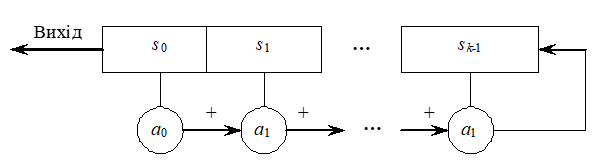
\includegraphics[width=0.75\linewidth]{templates/1-number-theory/register.png}
\end{tcolorbox}

\newpage
\section*{Задачі}
\subsection{Ентропія}
\begin{tcolorbox}[lowerbox=invisible,colback=white]
    \begin{minipage}{0.1\textwidth}
        \raggedright
        \vspace*{\fill}
            \textbf{Q1}
        \vspace*{\fill}
        \end{minipage}
        \begin{minipage}{0.75\textwidth}
       В урні лежать $6$ чорних та $9$ білих кульок. Виймають одну за одною дві кульки випадковим чином без повернення. Нехай $X$ означає колір першої кульки, $Y$ -- другої. Обчислити взаємну інформацію $I(X,Y)$.
        \end{minipage}
\end{tcolorbox}
\subsection{Лінійні регістри зсуву}
\begin{tcolorbox}[lowerbox=invisible,colback=white]
    \begin{minipage}{0.1\textwidth}
        \raggedright
        \vspace*{\fill}
            \textbf{Q2}
        \vspace*{\fill}
        \end{minipage}
        \begin{minipage}{0.75\textwidth}
        Нехай задано характеристичний поліном $$p(x)=x^4+x^3+x^2+x-1$$ над полем $F_2$, початковий стан $(s_0,s_1,s_2,s_4)=(1,0,0,1)$.
        \begin{itemize}
            \item Чому дорівнює період послідовності $T$, що породжена заданим за умовою початковим станом?
            \item Скільки унікальних послідовностей (циклів) може породити заданий поліном $p(x)$ (включно з тривіальними)? Випишіть їх.
            \item Якщо початковий стан $(s_0,s_1,s_2,s_4)=(1,0,0,1)$, визначіть яке буде значення ЛРЗ у 98 такті.
        \end{itemize}
        \end{minipage}
\end{tcolorbox}
\subsection{Схема Фейстеля та режими блокових шифрів}
\begin{tcolorbox}[lowerbox=invisible,colback=white]
    \begin{minipage}{0.1\textwidth}
        \raggedright
        \vspace*{\fill}
            \textbf{Q3}
        \vspace*{\fill}
        \end{minipage}
        \begin{minipage}{0.75\textwidth}
        Доведіть, що алгоритм розшифрування в схемі Фейстеля відрізняється від алгоритму шифрування лише зворотним порядком подачі циклових ключів
        \end{minipage}
\end{tcolorbox}
\begin{tcolorbox}[lowerbox=invisible,colback=white]
    \begin{minipage}{0.1\textwidth}
        \raggedright
        \vspace*{\fill}
            \textbf{Q4}
        \vspace*{\fill}
        \end{minipage}
        \begin{minipage}{0.75\textwidth}
        Розглянемо r-раундову схему Фейстеля, в якій раундова функція:
        \begin{align*}
           f_k(L,R)=R\oplus k.
        \end{align*} 
        Як за значенням блоку ШТ $Y$ знайти блок ВТ $X$ ? На виході якого раунду шифрування вперше з’явиться блок ВТ, якщо використовується один і той самий ключ?
        \end{minipage}
\end{tcolorbox}
\begin{tcolorbox}[lowerbox=invisible,colback=white]
    \begin{minipage}{0.1\textwidth}
        \raggedright
        \vspace*{\fill}
            \textbf{Q5}
        \vspace*{\fill}
        \end{minipage}
        \begin{minipage}{0.75\textwidth}
        Рядок бітів розбито на чотирьохбітові блоки і зашифровано блоковим
шифром, що заданий перестановкою 
\begin{align*}
    \pi=\left\{\begin{array}{сссс}
    1 & 2 & 3 & 4  \\
     4 & 3 & 1 & 2 \end{array}\right\}.
\end{align*}
Розшифруйте текст \texttt{101000011111} у режимах:
\begin{enumerate}
    \item OFB
    \item CFB
    \item CTR
\end{enumerate}
Вектор ініціалізації (синхропосилка) --- $IV=1001$.
        \end{minipage}
\end{tcolorbox}

\begin{tcolorbox}[lowerbox=invisible,colback=white]
    \begin{minipage}{0.1\textwidth}
        \raggedright
        \vspace*{\fill}
            \textbf{Q6}
        \vspace*{\fill}
        \end{minipage}
        \begin{minipage}{0.75\textwidth}
       Чотирибітовий блоковий шифр E задається формулою
$E(x_1, x_2, x_3, x_4) = (x_2 \oplus x_1, x_3, x_4, x_1)$.
Зашифруйте повідомлення $P = \texttt{1010101010}$ у режимі OFB, СВС, $IV = 1100$.
\end{minipage}
\end{tcolorbox}
\begin{tcolorbox}[lowerbox=invisible,colback=white]
    \begin{minipage}{0.1\textwidth}
        \raggedright
        \vspace*{\fill}
            \textbf{Q7}
        \vspace*{\fill}
        \end{minipage}
        \begin{minipage}{0.75\textwidth}
Сімейство блокових шифрів MISTY побудовано на основі схеми шифрування (так званої L-схеми), в якій один раунд має вид:
\begin{align*}
    F_k(x,y)=(y,y\oplus f_k(x))
\end{align*}
Накресліть схеми шифрування та розшифрування (один раунд). Чи буде ця схема інволютивною при зворотній подачі ключів? Чи обов’язково функція $f$ має бути бієкцією?
    \end{minipage}
\end{tcolorbox}

\begin{tcolorbox}[lowerbox=invisible,colback=white]
    \begin{minipage}{0.1\textwidth}
        \raggedright
        \vspace*{\fill}
            \textbf{Q8}
        \vspace*{\fill}
        \end{minipage}
        \begin{minipage}{0.75\textwidth}
       При передачі по каналу зв’язку тексту, зашифрованого блоковим шифром у
режимі ОFВ, був спотворений один блок ШТ. Які зміни відбудуться у ВТ
після розшифрування? А якщо один блок ШТ випав?
        \end{minipage}
\end{tcolorbox}

\begin{figure}
    \centering
    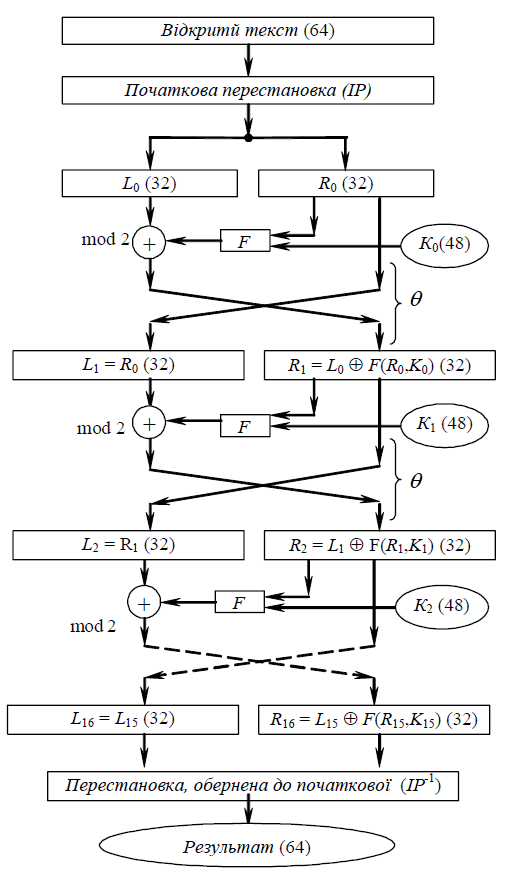
\includegraphics[width=0.5\linewidth]{4-crypto-practice/images/Feistel_scheme.png}
    \caption{Схема Фейстеля. Приклад на основі схеми DES}
    \label{fig:placeholder}
\end{figure}


\end{document}